%%%%%%%%%%%%%%%%%%%%%%%%%%%%%%%%%%%%%%%%%%%%%%%%%%%
%% P3: Phenomenology of Particle Physics                         
%%
%% Author:  André Rubbia                   		 
%%
%% Figure 11.19 Compton scattering formula:  angular distribution of the scattered photon.
%%
%% This work is licensed under the Creative Commons Attribution 4.0 International License. 
%% To view a copy of this license, visit http://creativecommons.org/licenses/by/4.0/ or 
%% send a letter to Creative Commons, PO Box 1866, Mountain View, CA 94042, USA.
%%
%%%%%%%%%%%%%%%%%%%%%%%%%%%%%%%%%%%%%%%%%%%%%%%%%%%

\documentclass[a4paper,10pt]{article}

\usepackage[T1]{fontenc}
\usepackage[utf8]{inputenc}
\usepackage{lmodern}
\usepackage[labelfont=bf]{caption}
\usepackage{upgreek}

\usepackage{tikz}
\usepackage{pgfplots}
\pgfplotsset{compat=1.17}
\usepgfplotslibrary{ternary}
\usepgfplotslibrary{fillbetween}
\usepgfplotslibrary{external}

\usepackage{braket}

\def\d{\mathrm{d}}

\begin{document}

%%%%%%%%%%%%%%%%% FIGURE %%%%%%%%%%%%%%%%%%%%%%%%%%%%%%%%%%
\begin{figure}[htb]
\begin{center}
\pgfplotsset{every axis/.append
    style={
    line width=1pt,
    tick style={line width=0.8pt}}}
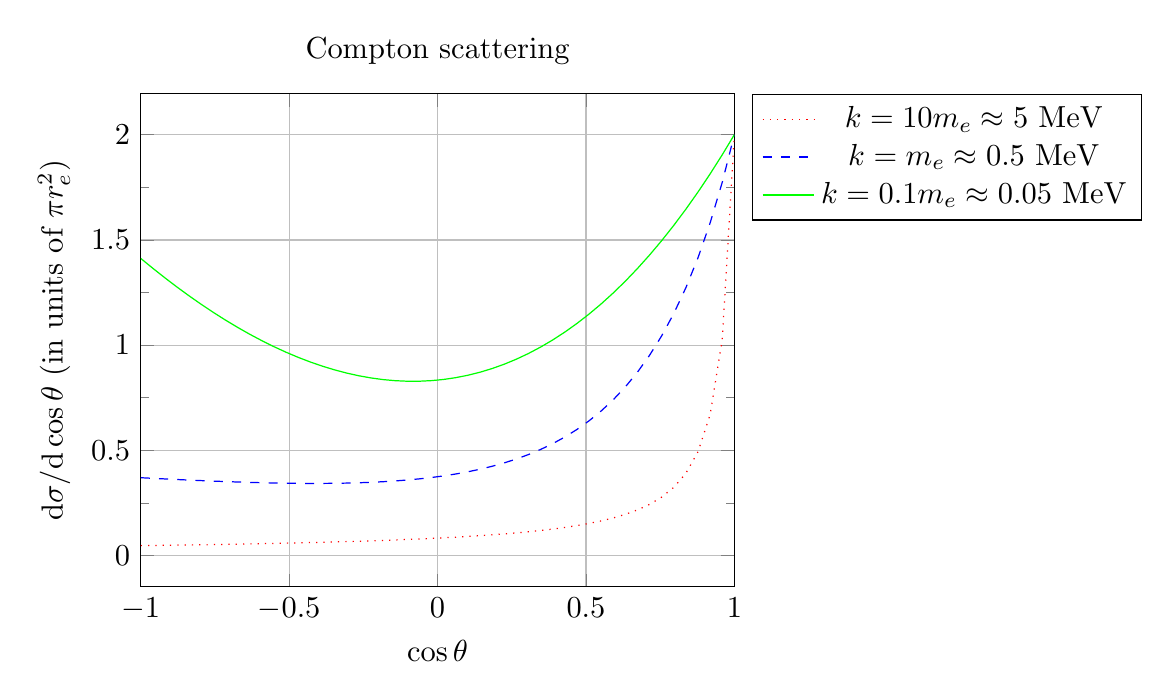
\begin{tikzpicture}[scale=1.1]
    \begin{axis}[
        title=Compton scattering,
        xlabel={$\cos\theta$},
        ylabel={$\d \sigma/\d \cos\theta$ (in units of $\pi r_e^2$)},
        xmin=-1, xmax=1,
        minor y tick num=1,
        grid = major,
        legend entries={
        $k=10m_e\approx 5$~MeV,
        $k=m_e\approx 0.5$~MeV,
        $k=0.1m_e\approx 0.05$~MeV,
        },
                legend style={legend pos = outer north east}
    ]
        \newcommand\ALPHA{(10)}
        \addplot [red,samples=50,domain=-1:1, dotted]
        {(1/(1+\ALPHA*(1-x))^2*(1+x^2+(\ALPHA^2*(1-x)^2)/(1+\ALPHA*(1-x)))};
        \renewcommand\ALPHA{(1)}
        \addplot [blue,samples=50,domain=-1:1, dashed]
        {(1/(1+\ALPHA*(1-x))^2*(1+x^2+(\ALPHA^2*(1-x)^2)/(1+\ALPHA*(1-x)))};
        \renewcommand\ALPHA{(0.1)}
        \addplot [green,samples=50,domain=-1:1]
        {(1/(1+\ALPHA*(1-x))^2*(1+x^2+(\ALPHA^2*(1-x)^2)/(1+\ALPHA*(1-x)))};
   \end{axis}
\end{tikzpicture}%
\caption{Compton scattering formula:  angular distribution of the scattered photon for various
incoming energies.}
\end{center}
\end{figure}
%%%%%%%%%%%%%%%%% END FIGURE %%%%%%%%%%%%%%%%%%%%%%%%%%%%%%
%

\end{document}
